
\section{\bfseries 研究目标}

围绕时空混合离散分析方法目前不适用于非结构型网格和稳定性机理不清晰的两大科学问题，本项目旨在发展\textbf{适用于非结构性网格的完全弱形式无网格增稳时空混合离散分析方法}，具体的研究目标如下：

(1) \textbf{时间末端虚位移边界条件的施加方法}。
为构造时间和空间维度上完全弱形式的时空混合离散方法，不可避免地需要施加时间末端虚位移边界条件。
进而使所提方法适用于非结构型网格、自适应节点加密过程及移动边界问题。

(2) \textbf{基于最优自由度配比的稳定无网格时空混合离散方案}。
该方案将利用再生核无网格近似离散的便利性，调整位移-动量自由度配比以消除数值色散引起的稳定性问题，使所提方法使用于非结构型网格的同时，提升计算精度。

(3) \textbf{基于赫林格-赖斯纳原理的变分一致时空混合离散伽辽金弱形式}。
由于研究目标(2)中所提的基于最优自由度配比的稳定时空混合离散方案将额外引入动量变量，在双变量混合离散框架下需要采用变分一致的伽辽金弱形式及本质边界条件施加方案，以保证计算结果的完备性。

(4) \textbf{高维变分一致时空混合离散伽辽金无网格数值积分方案}。
针对时空混合离散伽辽金弱形式中高维（四维）空间积分的计算效率问题，拟引入基于再生光滑梯度理论框架的数值积分方案，并利用数值积分点在单元间的共享特性优化全局积分点数，提升计算效率。

\section{\bfseries 具体研究内容和研究方案}

\subsubsection*{\bfseries (1) 时域末端虚位移本质边界条件施加方法}
首先，查阅基于哈密顿变分原理时空混合离散有限元法的相关文献，确定虚位移本质边界条件的几种可能性。
将不同虚位移边界的方法进行数值实现，对比计算结果的稳定性和精度。
确定稳定性最优情况下的虚位移空间$\tilde V_h$，相对应的变分问题为：
\begin{equation}
    \text{find} \; u_h \in V_h, \quad a(u_h, \delta u_h) = f(\delta u_h), \quad \forall \delta u_h \in \tilde V_h
    \label{eq:1}
\end{equation}
其中，$V_h$为位移空间，$a:V\times V \rightarrow \mathbb R$为双线性算子，$f:V\rightarrow \mathbb R$为线性算子。

随后，将式\eqref{eq:1}中的虚位移$\delta u_h$作为拉格朗日乘子，设计全新拉格朗日乘子型能量泛函：
\begin{equation}
    \text{find} \; u_h \in V_h,\; v_h \in \tilde V_h, \quad
    \left \{
    \begin{split} 
        -a(u_h, \delta u_h) + a(v_h, \delta u_h) = 0,\quad &\forall \delta u_h \in V_h \\
        a(u_h, \delta v_h) = f(\delta v_h),\quad &\forall \delta v_h \in \tilde V_h
    \end{split}
    \right .
    \label{eq:2}
\end{equation}
从上式可以看出，原本式\eqref{eq:1}中的变分问题作为约束条件施加在拉格朗日乘子型伽辽金问题的弱形式中，需进一步在验证两者之间的等价性。
当等价性成立，仅需要采用常规方法对$v_h$施加本质边界条件，即可实现式\eqref{eq:1}中施加虚位移本质边界条件的效果。
同时，引入分部积分公式对式\eqref{eq:2}进行推导，通过修正$u_h$和$v_h$的边界条件，使所提的拉格朗日乘子型伽辽金弱形式满足变分一致性，并证明其与欧拉--拉格朗日方程等价。

最后，采用均布的有限元离散结合罚函数法施加边界条件，从数值上与传统方法进行对比，验证其计算精度。并用分均布节点离散验证所提方法求解的稳定性。

\subsubsection*{\bfseries (2) 基于最优自由度配比的稳定无网格时空混合离散方案}

首先，在哈密顿原理中引入勒让德变换，将以位移为变量的能量泛函转化为位移-动量双变量的能量泛函。
并对其进行变分，从而建立位移-动量混合离散伽辽金弱形式。
该弱形式为广义鞍点问题，采用泛函分析手段对其进行误差估计，并分析LBB稳定性条件及其稳定系数在求解稳定性中的影响机理。

随后，采用完备多项式预估法\cite{}进一步分析位移-动量混合离散伽辽金弱形式的LBB稳定性条件。
探究位移和动量自由度数量对该弱形式求解稳定性的影响，建立基于位移-动量自由度配比的LBB稳定系数估计表达式，并从理论上分析最优自由度配比条件。

最后，在伽辽金弱形式中分别引入有限元近似、再生核无网格近似离散位移、动量，建立离散控制方程。
并采用具有精确解的传统波动方程数值算例（如简谐波问题）验证所提的基于最优自由度配比的稳定时空混合离散方案在非结构型网格下计算精度和稳定性。
其中，为规避时域末端边界条件的影响，所有边界均按精确解施加本质本质边界条件。

\subsubsection*{\bfseries (3) 满足变分一致性的时空混合离散伽辽金弱形式}

首先，在赫林格-赖斯纳变分原理的框架下，对位移-动量双变量能量泛函进行重新调整，其中时间维度作为第四维空间维度进行处理。
对调整后的能量泛函进行变分，可得相对应的时空混合离散伽辽金弱形式。
该弱形式在赫林格-赖斯纳变分原理的框架下将自动包含本质边界条件项，同时将满足变分一致性。

随后，采用再生光滑梯度理论框架\cite{}将动量转为位移自由度表示的再生梯度近似，而伽辽金弱形式也将转为单变量形式。
此时，即可将研究方案(1)中所提的时域末端虚位移边界条件施加方案引入其中，在该框架下虚位移本质边界条件与位移边界条件将得以协同施加，不起冲突。

最后，通过典型波动方程二维与三维算例（空间维度为一维和二维）系统验证所提变分一致性、稳定性和误差收敛特性，探究位移本质边界条件施加过程是否需要引入罚函数稳定项稳定计算结果。

\subsubsection*{\bfseries (4) 时空混合离散下变分一致型伽辽金无网格数值积分方案}
首先，根据时空混合离散无网格近似中基向量的元素，推导拉格朗日型伽辽金弱形式的积分约束条件。
引入申请人所提出的再生光滑梯度理论框架，构建满足满足积分约束条件无网格形函数再生光滑梯度，以形函数的一阶时间光滑导数为例，其表达式为：
\begin{equation}
    \tilde \Psi_{I,t}(\boldsymbol x) = \boldsymbol p^{[n_x,n_t - 1]}(\boldsymbol x) \boldsymbol G^{ - 1} \boldsymbol g_{tI}
\end{equation}
其中，$\boldsymbol G$为矩量矩阵，$\boldsymbol g_{tI}$为积分约束条件。再生光滑梯度能自动满足变分一致性条件，适用于相对应阶次的高斯积分方案。

随后，为进一步提升计算效率，将根据再生光滑梯度的一致性条件和数值积分点在单元间的共享特性，优化数值积分点的位置和权重，减少全局数值积分点数量。特别是针对四维空间，拟采用如图 \ref{fg:domain} 所示四面体柱或六面体柱单元作为背景积分域进行数值积分，构建适合时空混合离散再生光滑梯度积分法的数值积分方案。

% \vspace{20pt}
% \begin{figure}[!h]
%     \centering 
%     \subfloat[四面体柱积分域]{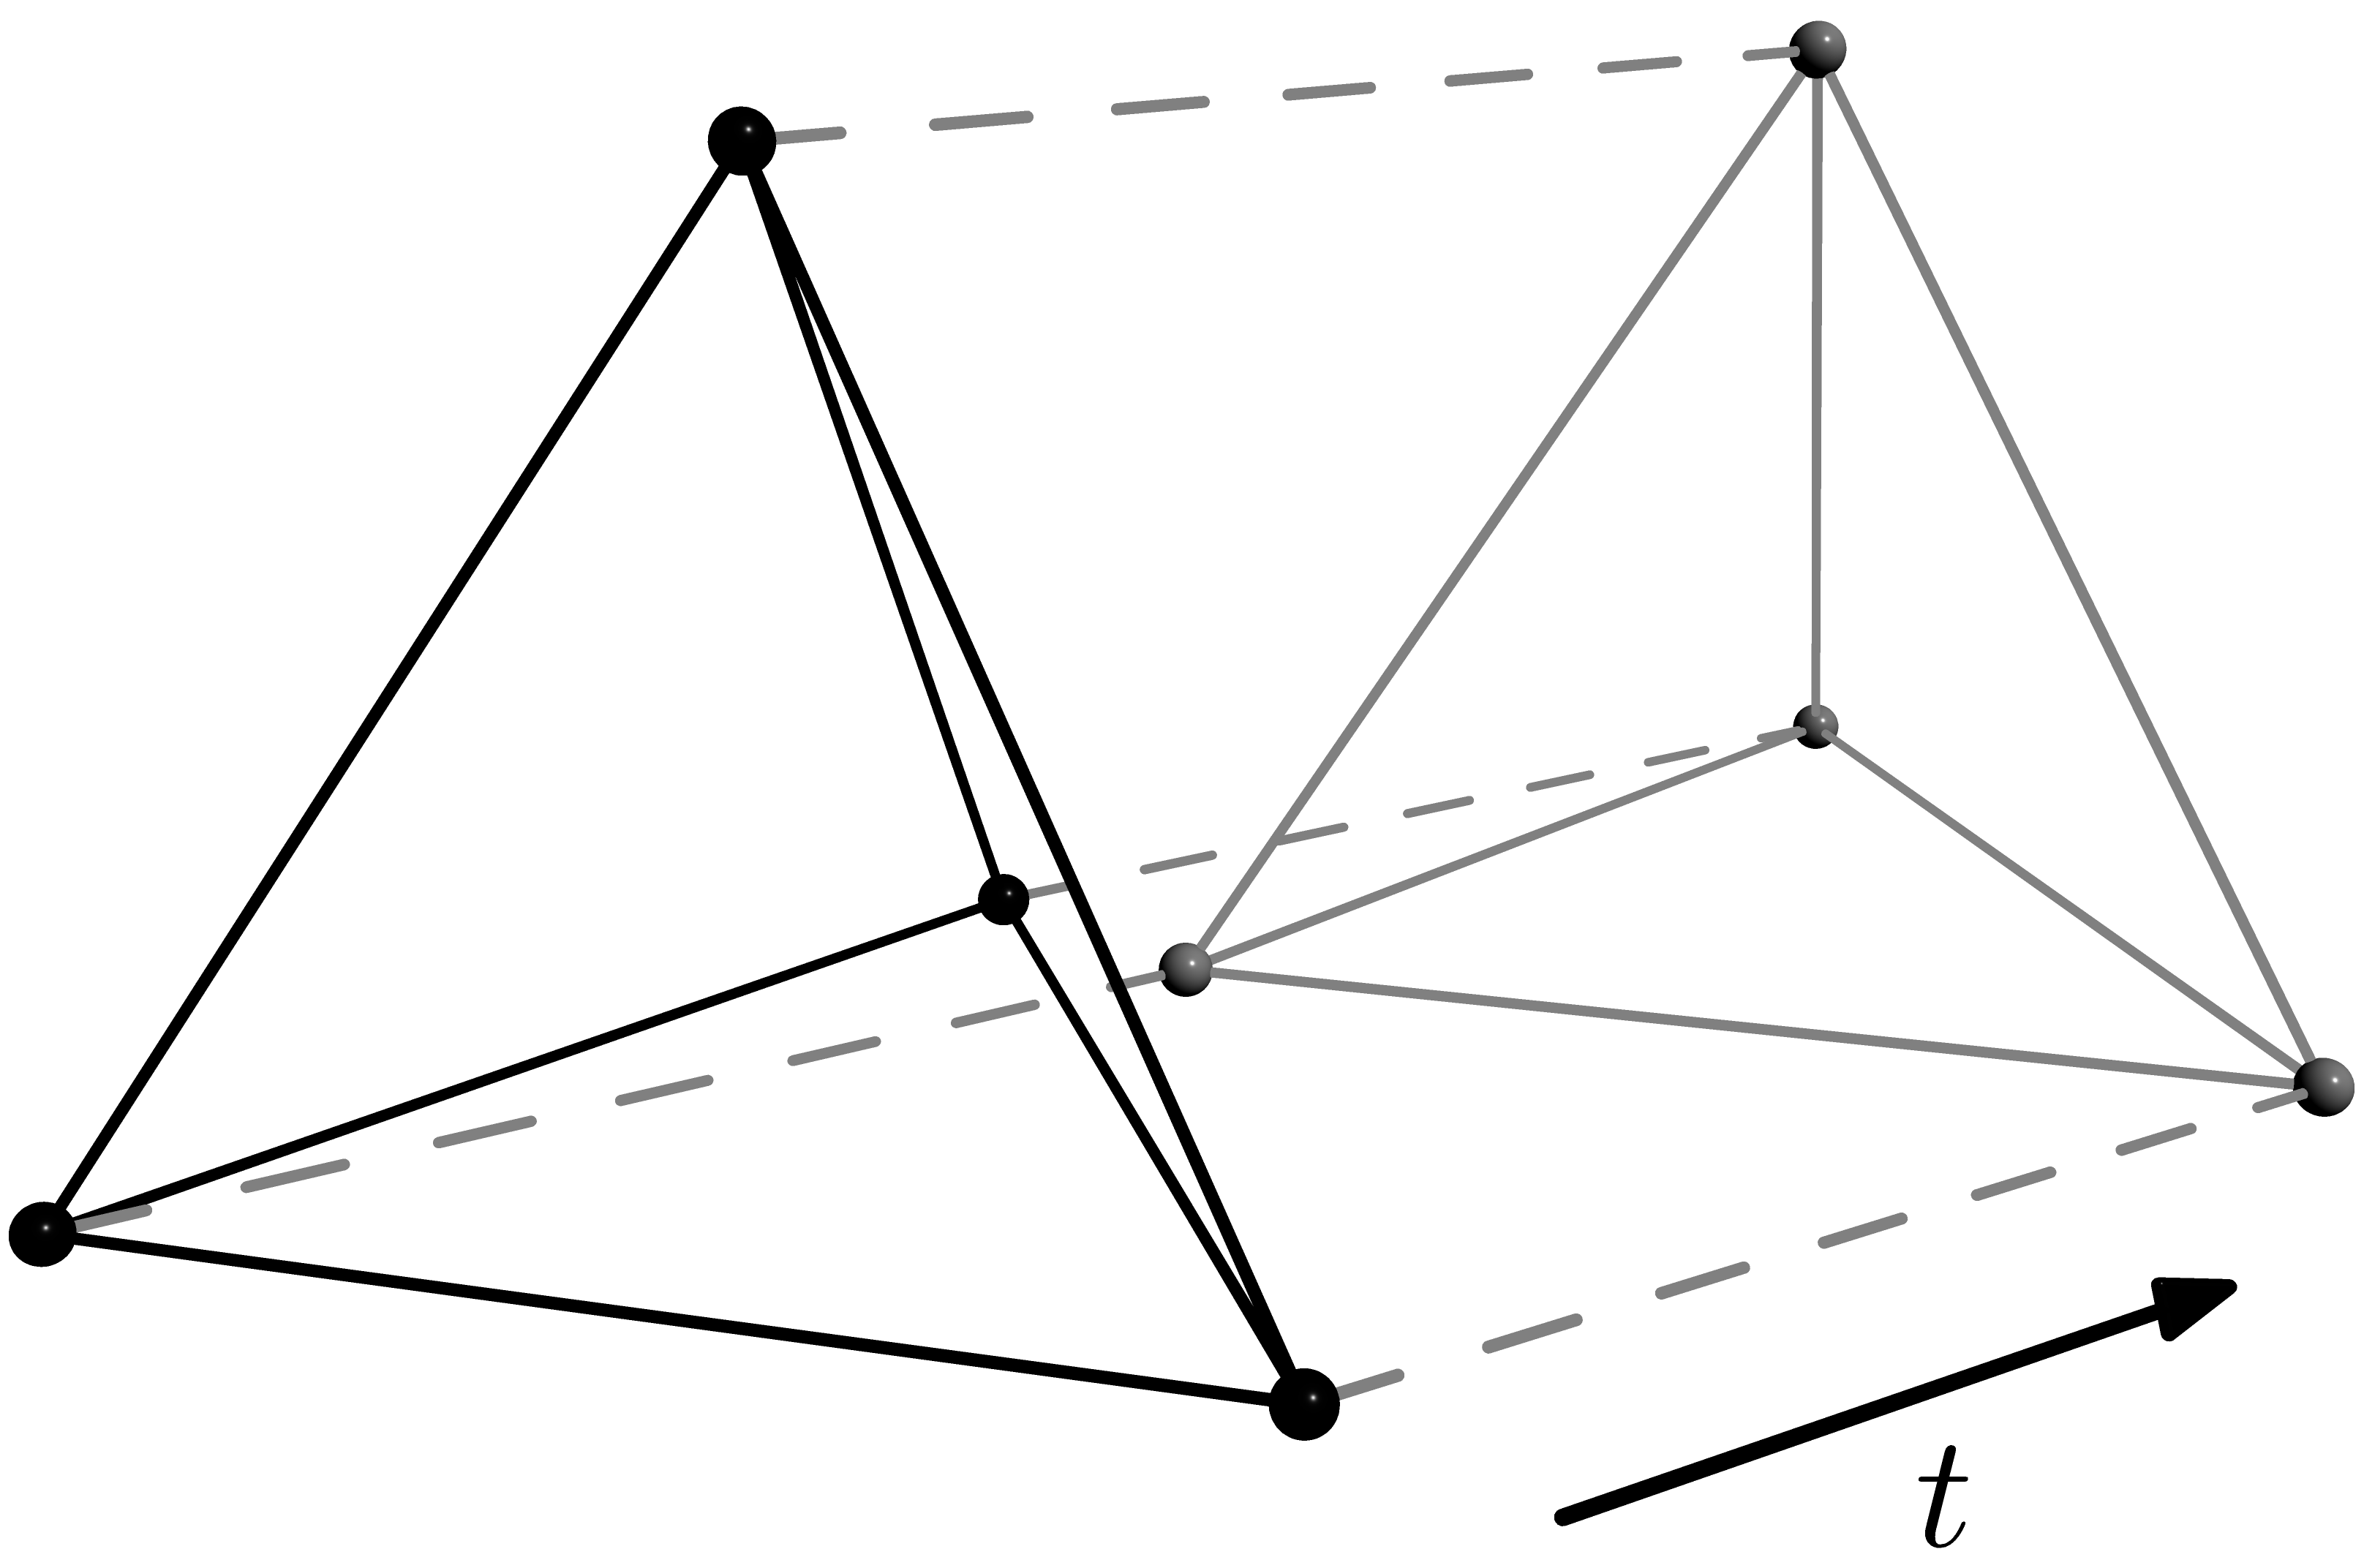
\includegraphics[width=0.4\textwidth]{figures/tetraprism_new.png}\label{fg:tet_domain}}
%     \hspace{24pt}
%     \subfloat[六面体柱积分域]{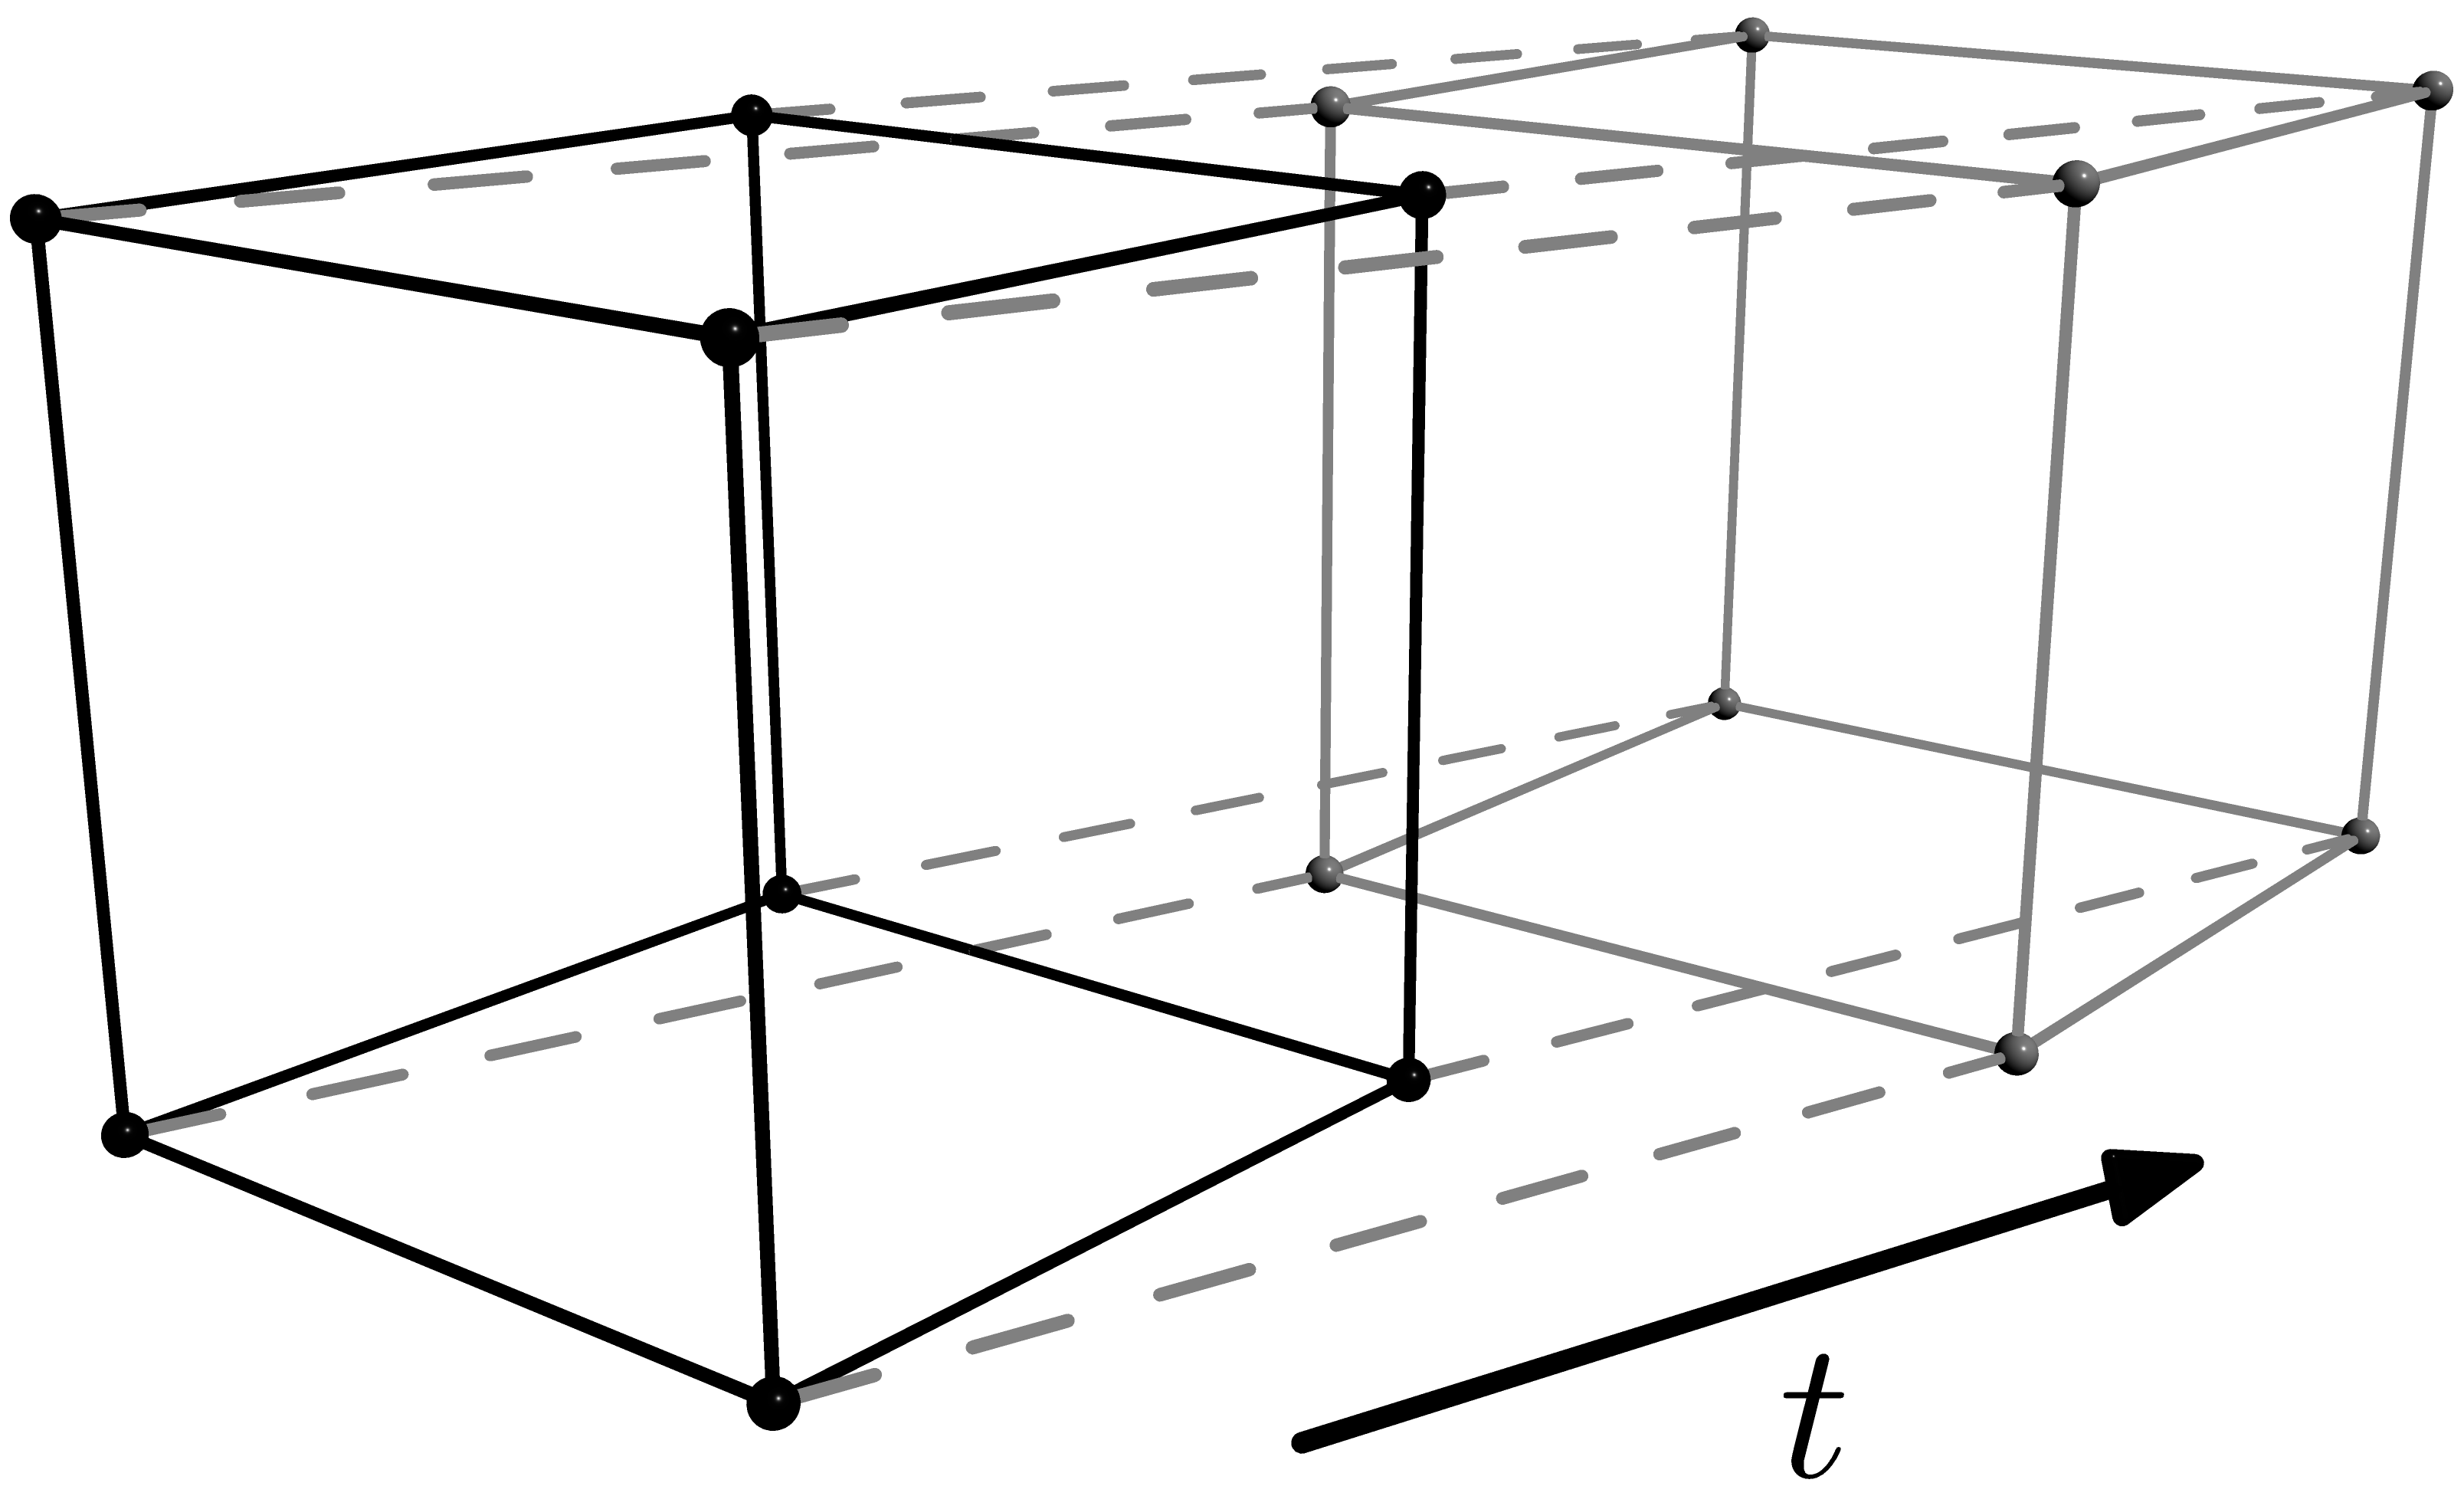
\includegraphics[width=0.4\textwidth]{figures/cubeprism_new.png}\label{fg:hex_domain}}
%     \caption{四维空间背景积分域}
%     \label{fg:domain}
% \end{figure}

最后，通过分片试验验证所提数值积分方案是否满足变分一致性，同时利用典型波动问题测试其计算精度。

\section{\bfseries 特色与创新点}

\subsubsection*{\bfseries (1) 特色}

\begin{itemize}[left=24pt]
    \item \textbf{聚焦非结构网格的适用性}。
    目前时空混合离散分析方法由于时间末端边界条件施加困难，导致现有方法采用结构网格或半结构网格（空间维度平行）。
    本项目将提出的时间末端虚位移边界条件施加方法，使得时空混合离散分析方法可适用于非结构网格，提升该方法在时空自适应节点加密、移动边界问题等方面的应用潜力。
    \item \textbf{从广义鞍点问题的LBB稳定性条件考虑数值色散的稳定性机理}。
    传统迭代求解动力问题的方法主要通过控制时间步长和空间网格尺寸来满足数值稳定性条件，如CFL条件。
    而时空混合离散分析方法虽然也通过引入稳定项抑制数值色散的振荡现象，如SUPG/GLS方法，但其稳定性机理尚不清晰。
    本项目将从广义鞍点问题的LBB稳定性条件出发，采用完备多项式预估法分析时空混合离散分析方法的稳定性机理，提出基于位移-动量自由度配比的最优稳定性条件，从理论上指导数值色散的抑制。
\end{itemize}

\subsubsection*{\bfseries (2) 创新点}

\begin{itemize}[left=24pt]
    \item \textbf{拉格朗日乘子型时间末端虚位移边界条件施加方法}。
    该方法将虚位移作为拉格朗日乘子引入能量泛函中，构建了施加时间末端虚位移边界条件的路径，使得时空混合离散分析方法可适用于非结构网格。

    \item \textbf{具有最优自由度配比无网格增稳时空混合离散方案}。
    该方案将利用再生核无网格近似离散的便利性，调整位移-动量自由度配比以消除数值色散引起的稳定性问题，使所提方法使用于非结构型网格的同时，提升计算精度。
\end{itemize}

\section{年度研究计划}

本项目围绕拟定的研究目标，通过理论推导和数值验证的方法研究任意节点分布的时空混合离散伽辽金无网格法。
根据各部分研究内容的逻辑关系，制定了表 \ref{tb:plan} 所示的项目的年度计划表。
其中，成果整理、论文发表及年度报告贯穿执行期。
项目参与人执行期内计划参加学术会议并作项目相关报告不少于每年2人次。

\begin{table}[!h]
\caption{年度研究计划表}\label{tb:plan}
\centering
\begin{ganttchart}[
    % inline,
    % bar inline label anchor = north,
    include title in canvas=false,
    x unit = 8pt,
    y unit title = 14pt,
    hgrid={*1{draw=black!5, line width=.75pt}},
    vgrid={*1{draw=black!5, line width=.75pt}},
    canvas/.append style={fill=none,draw=black!20,line width=.75pt},
    title/.style={draw=black!5, fill=none},
    title height=1,
    bar height = 0.3,
    group height=.1,
    % title label node/.append style={below=0pt},
    newline shortcut=true,
    % bar label node/.append style={align=left, anchor=north},
    bar/.append style={fill=blue!50, rounded corners=4pt, draw=none},
    group label node/.append style={align=left, left=-.5cm, text width=17em},
    bar label node/.append style={left=0cm,align=left,text width=15em},
]{1}{32}
    \gantttitle{2026}{8}
    \gantttitle{2027}{8}
    \gantttitle{2028}{8}
    \gantttitle{2029}{8} \\
    \gantttitle{上半年}{4}
    \gantttitle{下半年}{4}
    \gantttitle{上半年}{4}
    \gantttitle{下半年}{4}
    \gantttitle{上半年}{4}
    \gantttitle{下半年}{4}
    \gantttitle{上半年}{4}
    \gantttitle{下半年}{4} \\
    \ganttgroup{\bfseries 研究内容（1）}{1}{8} \\
    \ganttbar{查阅相关文献，测试不同虚位移边界条件时空混合离散伽辽金法性能}{1}{4}\\
    \ganttbar[name=scheme1]{研究拉格朗日乘子型时域末端虚位移本质边界条件施加方案}{3}{8}\\
    \ganttgroup{\bfseries 研究内容（2）}{9}{20} \\
    \ganttbar[name=error]{推导稳定性分析局部截断误差估计}{9}{20} \\
    \ganttbar[name=scheme2]{构建时空混合离散再生核近似方案}{13}{16} \\
    \ganttgroup{\bfseries 研究内容（3）}{17}{26} \\
    \ganttbar[name=scheme3]{推导时空混合离散再生光滑梯度}{17}{24} \\
    \ganttbar[name=scheme4]{优化四维积分域再生光滑梯度积分方案}{21}{26} \\
    \ganttgroup{\bfseries 研究内容（4）}{21}{28} \\
    \ganttbar[name=method]{构建时空混合离散伽辽金无网格法}{21}{24} \\
    \ganttbar{引入自适应节点分布算法和并行计算优化程序}{23}{28} \\
    \ganttbar{成果整理、论文发表、软件著作权申请、年度报告及项目结题报告}{5}{32}
\end{ganttchart}
\end{table}